\documentclass[11pt]{article}
\usepackage{amsmath,amsbsy,amssymb,verbatim,fullpage,ifthen,graphicx,bm,amsfonts,amsthm,url}
\usepackage{graphicx}
\usepackage{xcolor}
\usepackage{algorithm,algpseudocode}
\usepackage{xspace}
\usepackage{float}
\newcommand{\mfile}[1]  {{\small \verbatiminput{./#1}}} % Jeff Fessler, input matlab file
\newcommand{\tmop}[1]{\ensuremath{\operatorname{#1}}}
%\newcommand*{\qed}{\hfill\ensuremath{\blacksquare}}%
\newcommand{\R}{\mathbb{R}}
\newcommand{\C}{\mathbb{C}}
\newcommand{\Z}{\mathbb{Z}}
\newcommand{\A}{\mathcal{A}}
\newcommand{\minimize}{\operatorname*{minimize\ }}
\newcommand{\maximize}{\operatorname*{maximize}}
\newcommand{\opdet}[1]{\operatorname{\textbf{det}}\left(#1\right)}
\newcommand{\optr}[1]{\operatorname{\textbf{tr}}\left(#1\right)}
\newcommand{\AnswerDefine}{}
\newcommand{\answer}[2][blue]{\ifdefined\AnswerDefine{\color{#1}\it#2}\fi}
\newcommand{\mtx}[1]{\mathbf{#1}}
\newcommand{\vct}[1]{\mathbf{#1}}
\def \lg       {\langle}
\def \rg       {\rangle}
\def \mA {\mtx{A}}
\def \mB {\mtx{B}}
\def \mD {\mtx{D}}
\def \mE {\mtx{E}}
\def \mF {\mtx{F}}
\def \mG {\mtx{G}}
\def \mI {\mtx{I}}
\def \mJ {\mtx{J}}
\def \mL {\mtx{L}}
\def \mU {\mtx{U}}
\def \mS {\mtx{S}}
\def \mV {\mtx{V}}
\def \mW {\mtx{W}}
\def \mLambda {\mtx{\Lambda}}
\def \mSigma {\mtx{\Sigma}}
\def \mX {\mtx{X}}
\def \mY {\mtx{Y}}
\def \mZ {\mtx{Z}}
\def \zero     {\mathbf{0}}
\def \vzero    {\vct{0}}
\def \vone    {\vct{1}}
\def \va {\vct{a}}
\def \vg {\vct{g}}
\def \vm {\vct{m}}
\def \vu {\vct{u}}
\def \vv {\vct{v}}
\def \vw {\vct{w}}
\def \vx {\vct{x}}
\def \vy {\vct{y}}
\def \vz {\vct{z}}
\def \vphi {\vct{\phi}}
\def \vmu {\vct{\mu}}
\def \R {\mathbb{R}}

%\newcommand{\st}{\operatorname*{\ subject\ to\ }}
\usepackage{algorithm,algpseudocode}
\usepackage{xspace}
% Add a period to the end of an abbreviation unless there's one
% already, then \xspace.
\makeatletter
\DeclareRobustCommand\onedot{\futurelet\@let@token\@onedot}
\def\@onedot{\ifx\@let@token.\else.\null\fi\xspace}

\def\eg{\emph{e.g}\onedot} \def\Eg{\emph{E.g}\onedot}
\def\ie{\emph{i.e}\onedot} \def\Ie{\emph{I.e}\onedot}
\def\cf{\emph{c.f}\onedot} \def\Cf{\emph{C.f}\onedot}
\def\etc{\emph{etc}\onedot} \def\vs{\emph{vs}\onedot}
\def\wrt{w.r.t\onedot} \def\dof{d.o.f\onedot}
\def\etal{\emph{et al}\onedot} \def\st{\emph{s.t}\onedot}
\pagestyle{plain}

\title{{\bf Final Exam, CPSC 8420, Spring 2022}} 
\author{\Large\underline{Huang, Gangtong}}% put your name in the LastName, FirstName format
\date{\textbf{\Large\textcolor{red}{Due 05/06/2022, Friday, 11:59PM EST}}} 
%\date{\today}

\begin{document}
\maketitle

\section*{Problem 1 [15 pts]}
Consider the elastic-net optimization problem:
\begin{equation}
\min_{\beta} \|\vy-\mX\beta\|^2+\lambda[\alpha\|\beta\|^2_2+(1-\alpha)\|\beta\|_1].
\end{equation}
\begin{enumerate}
	\item Show the objective can be reformulated into a lasso problem, with a slightly different $\mX, \vy$.\\ \\
	Define: 
	$
	\mX_1=
	(1+\lambda\alpha)\begin{pmatrix}
		\mX \\
		\sqrt{\lambda\alpha}\mI_p
	\end{pmatrix}
	$,  
	$
	\vy_1=\begin{pmatrix}
		\vy\\
		0
\end{pmatrix}
	$, and $\beta_1=\sqrt{1+\lambda\alpha}\beta$ then: 
	\begin{equation}
		\begin{aligned}
			\mX_1^T\mX_1&=(1+\lambda\alpha)(\mX^T\mX+\lambda\alpha\mI)\\
			&=(1+\lambda\alpha)(\mX^T\mX+\lambda\alpha)
		\end{aligned}
	\end{equation}, and
	\begin{equation}
		\begin{aligned}
			\vy_1^T\vy_1&=\vy^T\vy+0\\
			&=\vy^T\vy
		\end{aligned}
	\end{equation}
	Define $\mL(\vy_1,\mX_1,\beta_1)=\|\vy_1-\mX_1\beta_1\|^2 + \frac{\lambda(1-\alpha)}{1+\lambda\alpha}\|\beta_1\|_1$. Formulata a Lasso problem using $\mX_1$, $\vy_1$, $\beta_1$: 
	\begin{equation}
		\min_{\beta_1}\mL(\vy_1,\mX_1,\beta_1)
	\end{equation}, where:
	
	\begin{equation}
		\begin{aligned}
			\mL(\vy_1,\mX_1,\beta_1) &= \|\vy_1-\mX_1\beta_1\|^2 + \frac{\lambda(1-\alpha)}{1+\lambda\alpha}\|\beta_1\|_1 \\
			&= (\vy_1-\mX_1\beta_1)^T(\vy_1-\mX_1\beta_1)+\frac{\lambda(1-\alpha)}{1+\lambda\alpha}\|\beta_1\|_1\\
			&= \vy_1^T\vy_1-\beta_1^T\mX^Ty_1-y_1^T\mX_1\beta+\beta_1^T\mX_1^T\mX_1\beta_1 + \frac{\lambda(1-\alpha)}{1+\lambda\alpha}\|\beta_1\|_1
		\end{aligned}
	\end{equation}
	Plug eqns. (2), (3) into eqn. (4), we will arrive at:
	\begin{equation}
	\mL(\vy_1,\mX_1,\beta_1) = \|\vy_1-\mX_1\beta_1\|^2 + \frac{\lambda(1-\alpha)}{1+\lambda\alpha}\|\beta_1\|_1 
	\end{equation}, and the optimization problem in eqn. (4) becomes: 
\begin{equation}
	\min_{\beta_1} \|\vy_1-\mX_1\beta_1\|^2 + \frac{\lambda(1-\alpha)}{1+\lambda\alpha}\|\beta_1\|_1 
\end{equation}, where the only difference with the original optimization problem is the variable $\beta_1$. Since $\beta_1=\sqrt{1+\lambda\alpha}\beta$, the optimization problem in eqn. (7) is equivalent to:
	\begin{equation}
		\min_{\beta} \|\vy_1-\mX_1\beta_1\|^2 + \frac{\lambda(1-\alpha)}{1+\lambda\alpha}\|\beta_1\|_1
	\end{equation}, which is the original objective function of the elastic net problem.

	\item If we fix $\alpha=.5$, please derive the closed solution by making use of alternating minimization that each time we fix the rest by optimizing one single element in $\beta$. You need randomly generate $\mX, \vy$ and initialize  $\beta_0$, and show the objective decreases monotonically with updates.\\ \\
	For the Lasso problem $\min_{\beta_1} \|\vy_1-\mX_1\beta_1\|^2 + \frac{\lambda(1-\alpha)}{1+\lambda\alpha}\|\beta_1\|_1$, the closed solution of the $i$-th element of $\beta_1$ is:
	\begin{equation}
		\begin{aligned}
			\beta_{1i} = signum(\beta_{1i}^{LS})(\|\beta_{i1}^{LS}\|_1-\frac{\lambda(1-\alpha)}{1+\lambda\alpha})^+
		\end{aligned}
	\end{equation}
, where $\beta_{i1}^{LS}=X_1^Ty_1$ is the solution of the vanilla least square problem.\\
Before the each time $beta_1^{i+1}-beta_1^{i}$ is evaluated against the tolerance, each component $beta_{1i}$ is optimized once. Fig. 1 shows the decrease of the objective function with the optimization of each single $\beta_{1i}$.
\begin{figure}[H] % This is how figure are placed into latex document
	\centering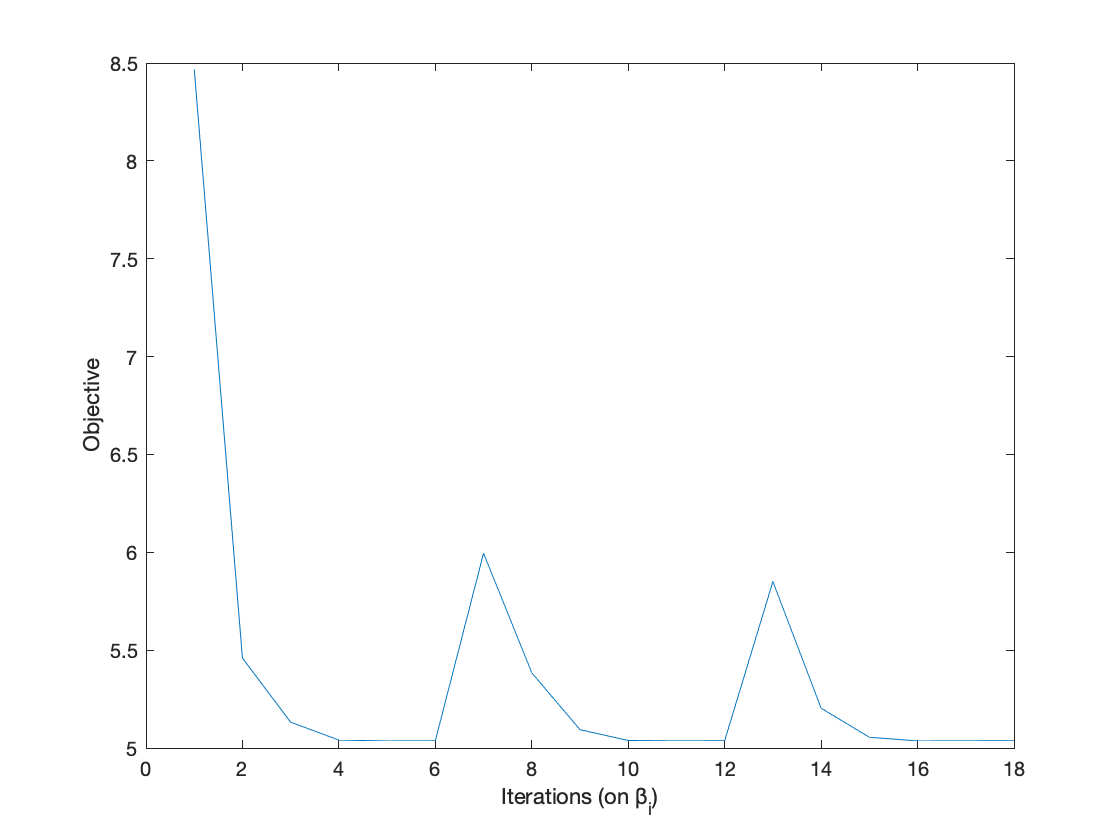
\includegraphics[width=0.8\linewidth]{fin_1_2.png}
	\caption{Decrease of $\mL(\vy_1,\mX_1,\beta_1) = \|\vy_1-\mX_1\beta_1\|^2 + \frac{\lambda(1-\alpha)}{1+\lambda\alpha}\|\beta_1\|_1$ with gradient descent w.r.t. each component of $\beta_1$.} % caption of the figure
	\label{fig:fig6}  % Label the figure so you can refer to it in text.
\end{figure}
\textbf{Codes (MatLab):}
\begin{verbatim}
n = 3;
m = 4;

lambda = 10;
alpha = 1/2;
gamma = lambda*(1-alpha)/(1+lambda*alpha)

X = rand(m,n);
y = 5 * rand(m,1);

Xcent = zscore(X);

X_1 = (1 + lambda*alpha) * [Xcent; eye(n)];
y_1 = [y; zeros(n,1)];

%% Output L in each step
mat_obj = lassoAlg_step(X_1, y_1, gamma)
l_obj = reshape(mat_obj,1,[])

plot(l_obj)
xlabel('Iterations (on beta_i)')
ylabel('Objective')

%%
lassoAlg(X_1, y_1, gamma);
%% Lasso Optimization Algorithm %%
% inputs: A (nxd matrix), y (nx1 vector), lam (scalar)
% return: xh (dx1 vector)

function xh = lassoAlg(A,y,lam)     
xnew = rand(size(A,2),1);   % "initial guess" 
xold = xnew+ones(size(xnew)); % used zeros so the while loop initiates
loss = xnew - xold;
thresh = 10e-3;     % threshold value for optimization

while norm(loss) > thresh
xold = xnew;    % need to store the previous iteration of xh
for i = 1:length(xnew)
a = A(:,i);     % get column of A
p = (norm(a,2))^2;
% from notes: -t = sum(aj*xj) - y for all j != i
% i.e., sum(aj*xj) - ai*xi - y (my interpretation)
% hence t = (above) * -1
% want to be sure this the correct definition of t?
t =  a*xnew(i) + y - A*xnew; 
q = a'*t;
% update xi
xnew(i) = (1/p) * sign(q) * max(abs(q)-lam, 0);
end
loss = xnew - xold;     % update loss 
end
xh = xnew;
end

%% Lasso Optimization Algorithm %%
% inputs: A (nxd matrix), y (nx1 vector), lam (scalar)
% return: xh (dx1 vector)

function xh = lassoAlg_step(A,y,lam)     
xnew = rand(size(A,2),1);   % "initial guess" 
xold = xnew+ones(size(xnew)); % used zeros so the while loop initiates
loss = xnew - xold;
thresh = 10e-3;     % threshold value for optimization
xh = [];

while norm(loss) > thresh
xold = xnew;    % need to store the previous iteration of xh
tmp = [];
for i = 1:length(xnew)
a = A(:,i);     % get column of A
p = (norm(a,2))^2;
% from notes: -t = sum(aj*xj) - y for all j != i
% i.e., sum(aj*xj) - ai*xi - y (my interpretation)
% hence t = (above) * -1
% want to be sure this the correct definition of t?
t =  a*xnew(i) + y - A*xnew; 
q = a'*t;
% update xi
xnew(i) = (1/p) * sign(q) * max(abs(q)-lam, 0);
obj = norm(y - A * xnew, 2) + lam*(1-1/2)/(1+lam*1/2)*norm(xnew,1);
tmp = [tmp, obj];
end
loss = xnew - xold;     % update loss 
%obj = norm(y - A * xnew, 2) + lam*(1-1/2)/(1+lam*1/2)*norm(xnew,1);
%xh = [xh, obj];
xh = [xh; tmp];
end
end
\end{verbatim}

		
\end{enumerate}
\answer{You may input your answers here. \LaTeX \ version submission is encouraged.}
\newpage
\section*{Problem 2 [15 pts]}
\begin{itemize}
	\item For PCA, the loading vectors can be directly computed from the $q$ columns of  $\mU$ where  $[\mU,\mS,\mU]=svd(\mX^T\mX)$, please show that any $[\pm\vu_1,\pm\vu_2,\dots,\pm\vu_q]$ will be equivalent to $[\vu_1,\vu_2,\dots,\vu_q]$ in terms of the same variance while satisfying the orthonormality constraint.\\ \\
	In PCA, the variance of the $i$-th principal component (PC) is: 
	\begin{equation}
		\begin{aligned}
			Var(u_i)&=\vu_i^T \mX^T\mX \vu_i \\
			&= \vu_i^Ts_i\vu_i\\
			&= s_i\vu_i^T\vu_i\\
			&= s_i
		\end{aligned}
	\end{equation}
	, where $s_i$ is the $i$-th singular value of $X$.\\
	Substituting $u_i$ with $-u_i$, we have:
	\begin{equation}
		\begin{aligned}
			Var(-u_i)&=(-\vu_i^T) \mX^T\mX (-\vu_i) \\
			&= (-\vu_i^T) s_i (-\vu_i)\\
			&= s_i\vu_i^T\vu_i\\
			&= s_i
		\end{aligned}
	\end{equation}
	, which is identical to the case of $u_i$.
	Also when $i\neq j$,
	\begin{equation}
		\begin{aligned}
			(-u_i)^Tu_j&=-u_i^Tu_j\\
			&=0
		\end{aligned}
	\end{equation}
	still satisfies orthonormality. \\
	So $Var(u_i)=Var(-u_i)$, and any sign combination of $[\vu_1,\vu_2,\dots,\vu_q]$ preserves the variance as well as orthonormality.
	
	\item We consider the case when original dimensionality of the data is much larger than the number of samples $d\gg m$ ($\mX\in\R^{m\times d}$). What's the complexity of obtaining the optimal solution of PCA via Singular Value Decomposition? Please consider a more efficient solution by considering the relationships of eigenvalues/eigenvectors between $\mX^T\mX$
	 and $\mX\mX^T$.\\ \\
	 Since $\mX\in\R^{m\times d}$, the complexity of $X^TX$ is: $O(d\times d\times m)=O(d^2m)$. Since $X^TX\in \R^{d\times d}$ is a square matrix, the complexity of $SVD(X^TX)$ is $O(d^3)$. Therefore, the complexity of PCA on $X^TX$ is $O(d^2m + d^3)$.\\
	 We know that the non-zero eigenvalues of $X^TX$ and $XX^T$ are the same, and hence the non-zero singular values. Similar to $PCA(X^TX)$, we know that the time complexity of the PCA of $XX^T$ is $O(m^2d + m^3)$, which is smaller than $O(d^2m + d^3)$ when $d\gg m$. Therefore, to reduce computational cost, we can perform $PCA(XX^T)$ instead of $PCA(X^TX)$.
	 
	 
\end{itemize}


\newpage
\section*{Problem 3 [10 pts]}
Assume that in a community, there are $10\%$ people suffer from COVID. Assume $80\%$ of the patients come to breathing difficulty while $25\%$ of those free from COVID also have symptoms of shortness of breath. Now please determine that if one has breathing difficulty, what's his/her probability to get COVID? (\textit{hint}: you may consider Naive Bayes)\\\\
The conditional probability of getting shortness of breath $B$ given getting Covid $C$ is:
\begin{equation}
	P(B|C) = 0.8
\end{equation} 
The probability of shortness of breath without Covid ($nC$):
\begin{equation}
	P(B|nC)=0.25
\end{equation}
So the probability of getting shortness of breath is:
\begin{equation}
	\begin{aligned}
		P(B)&=P(B|C)P(C)+P(B|nC)P(nC)\\
		&=P(B|C)P(C)+P(B|nC)[1-P(C)]\\
		&=0.8\times 0.1 + 0.25\times 0.9\\
		&=0.305
	\end{aligned}
\end{equation}
The probability of getting Covid:
\begin{equation}
	P(C)=0.1
\end{equation}
From Naive Bayesian, the probability of Covid given shortness of breath is:
\begin{equation}
	\begin{aligned}
		P(C|B)&=\frac{P(B|C)P(C)}{P(B)}\\
		&=\frac{0.8\times 0.1}{0.305}\\
		&=0.262
	\end{aligned}
\end{equation}


\newpage
\section*{Problem 4 [20 pts]}
Recall the objective for \text{RatioCut}: $RatioCut(A_1,A_2,...A_k) = \frac{1}{2}\sum\limits_{i=1}^{k}\frac{W(A_i, \overline{A}_i )}{|A_i|}$. If we introduce indicator vector: $h_j \in \{h_1, h_2,..h_k\}, j \in [1,k]$, for any vector $h_j\in R^n$, we define: $h_{ij}= \begin{cases} 0& { v_i \notin A_j}\\ \frac{1}{\sqrt{|A_j|}}& { v_i \in A_j} \end{cases}$, we can prove: $h_i^TLh_i =  \frac{cut(A_i, \overline{A}_i)}{|A_i|}$, and therefore:
\begin{equation}
	RatioCut(A_1,A_2,...A_k) = \sum\limits_{i=1}^{k}h_i^TLh_i = \sum\limits_{i=1}^{k}(H^TLH)_{ii} = tr(H^TLH),
\end{equation}
thus we relax it as an optimization problem:
\begin{equation}
	\underbrace{arg\;min}_H\; tr(H^TLH) \;\; s.t.\;H^TH=I.
\end{equation}
Now let's explore Ncut, with objective:
$NCut(A_1,A_2,...A_k) = \frac{1}{2}\sum\limits_{i=1}^{k}\frac{W(A_i, \overline{A}_i )}{vol(A_i)}$, where $vol(A): = \sum\limits_{i \in A}d_i, d_i: = \sum\limits_{j=1}^{n}w_{ij}$.Similar to Ratiocut, we define: $h_{ij}= \begin{cases} 0& { v_i \notin A_j}\\ \frac{1}{\sqrt{vol(A_j)}}& { v_i \in A_j} \end{cases}$. Now
\begin{enumerate}
	\item Please show that $h_i^TLh_i =\frac{cut(A_i, \overline{A}_i)}{vol(A_i)}$.\\ \\
	\begin{equation}
		\begin{aligned}
			h_i^TLh_i &= \frac{1}{2}\sum_{m=1}\sum_{n=1}w_{mn}(h_{mi}-h_{ni})^2\\
			&= \frac{1}{2} [ \sum_{m\in A_i,n\notin A_i}(w_{mn}\frac{1}{\sqrt{vol(A_i)}} - 0)^2 + \sum_{m\notin A_i,n\in A_i}(0 - w_{mn}\frac{1}{\sqrt{vol(A_i)}})^2 + \\& \sum_{m\in A_i,n\in A_i}(w_{mn}\frac{1}{\sqrt{vol(A_i)}} - w_{mn}\frac{1}{\sqrt{vol(A_i)}})^2 + \sum_{m\notin A_i,n\notin A_i}(0 - 0) ]\\
			&=\frac{1}{2} [ \sum_{m\in A_i,n\notin A_i}\frac{w_{mn}}{vol(A_i)} + \sum_{m\notin A_i,n\in A_i} \frac{w_{mn}}{vol(A_i)} ]\\
			&=\frac{1}{2} [ \frac{cut(A_i,\bar{A_i})}{vol(A_i)} + \frac{cut(A_i,\bar{A_i})}{vol(A_i)} ]\\
			&=\frac{cut(A_i,\bar{A_i})}{vol(A_i)}
		\end{aligned}
	\end{equation}
	\item Show that $NCut(A_1,A_2,...A_k) = tr(H^TLH)$.\\ \\
	From the definition of Cut,
	\begin{equation}
		\begin{aligned}
			cut(A_1,A_2,...A_k) = \frac{1}{2}\sum\limits_{i=1}^{k}W(A_i,\bar{A_i})
		\end{aligned}
	\end{equation}
	From the result of Problem 4.1: $h_i^TLh_i = \frac{cut(A_i, \overline{A}_i)}{vol(A_i)}$, we have:
	\begin{equation}
		\begin{aligned}
			h_i^TLh_i &= \frac{cut(A_i, \overline{A}_i)}{vol(A_i)}\\
			&= \frac{1}{2} \frac{W(A_i,\bar{A_i})}{vol(A_i)}
		\end{aligned}
	\end{equation}
	So: 
	\begin{equation}
		\begin{aligned}
			NCut(A_1,A_2,...A_k) &= \frac{1}{2}\sum\limits_{i=1}^{k}\frac{W(A_i, \overline{A}_i )}{vol(A_i)}\\
			&= \sum\limits_{i=1}^{k} \frac{cut(A_i, \overline{A}_i)}{vol(A_i)}\\
			&= \sum\limits_{i=1}^{k} h_i^TLh_i \\
			&= \sum\limits_{i=1}^{k} (H^TLH)_{ii} \\
			&= tr(H^TLH)
		\end{aligned}
	\end{equation}
	
	
	\item The constraint now is: $H^TDH=I$.\\ \\
	\begin{equation}
		\begin{aligned}
			h_i^TDh_i &= \sum_{j}d_lh_{ji}^2\\
			&= \sum_{j\in A_i} d_l \frac{1}{vol(A_i)}\\
			&= \frac{1}{vol(A_i)} \sum_{j\in A_i} \sum_{m=1}^N w_{jm}\\
			&= 1
		\end{aligned}
	\end{equation}
	And since $(H^TDH)_{ii}=h_i^TDh_i$, all diagonal elements of $H^TDH$ are 1. Therefore, $H^TDH=\mI$.
	 
	\item Find the solution to $\underbrace{arg\;min}_H\; tr(H^TLH) \;\; s.t.\;H^TDH=I$.\\ \\
	Define a new matrix, $M$:
	\begin{equation}
		\begin{aligned}
			M=D^{\frac{1}{2}}H
		\end{aligned}
	\end{equation}
, where $D$ is the degree matrix, and thus $H=D^{-\frac{1}{2}}M$.
	Then, the minimization problem is equivalent to:
	\begin{equation}
		\begin{aligned}
			\min_{M} Tr(M^TD^{-\frac{1}{2}}LD^{-\frac{1}{2}}M)\\
			s.t. M^TM=I
		\end{aligned}
	\end{equation}
	, where $(D^{-\frac{1}{2}})^T=D^{-\frac{1}{2}}$, because the degree matrix $D$ is symmetrical. The problem can be further transformed into:
	\begin{equation}
		\begin{aligned}
			\min_{M} Tr(\frac{M^TD^{-\frac{1}{2}}LD^{-\frac{1}{2}}M}{M^TM})\\
			s.t. M^TM=I
		\end{aligned}
	\end{equation}
, in which form we can apply the Rayleigh-Ritz theorem, since all matrices in the problem are real matrices ($M^H=M^T$). We know that the minimun value of $\frac{M^TD^{-\frac{1}{2}}LD^{-\frac{1}{2}}M}{M^TM}$ is the smallest eigenvalue of $D^{-\frac{1}{2}}LD^{-\frac{1}{2}}$. Therefore, the solution of $M^T$ is a matrix that has the eigenvectors of $L$ as columns. By substituting $H=D^{-\frac{1}{2}}M$, we can get the solution of $H$.
	
\end{enumerate}

\newpage
\section*{Problem 5 [10 pts]}
We consider the following optimization problem ($\mY$ is given and generated randomly):
\begin{equation}
	\min_{\mX} \frac{1}{2}\|\mX-\mY\|^2_F + \|\mX\|_*
\end{equation}
where $\mY,\mX\in\R^{100\times100}$ and $\|\cdot\|_*$ denotes the nuclear norm (sum of singular values). Now please use gradient descent method to update $\mX$. ($\frac{\partial \|\mX\|_*}{\partial \mX}=\mU\mV^T$, where $\mU,\mV$ is obtained from reduced SVD, namely $[\mU,\mS,\mV]=svd(\mX,0)$). Plot the objective changes with 1000 iteration.\\ \\
The objective function is: $L(X,Y) = \frac{1}{2}\|X-Y\|_F^2+\|X\|_*$, and its derivative w.r.t. X is: 
\begin{equation}
	\begin{aligned}
		\frac{\partial L}{\partial X} = \frac{1}{2}(X-U) + UV^T\\
		& = X-Y+UV^T
	\end{aligned}
\end{equation}
, where $[U,S,V]=SVD_{red}(X)$ are derived from the reduced SVD of X.\\
The change of objective function L w.r.t. number of iterations in gradient descent method is shown in Fig. 1. Codes implemented with MatLab.
\begin{figure}[H] % This is how figure are placed into latex document
	\centering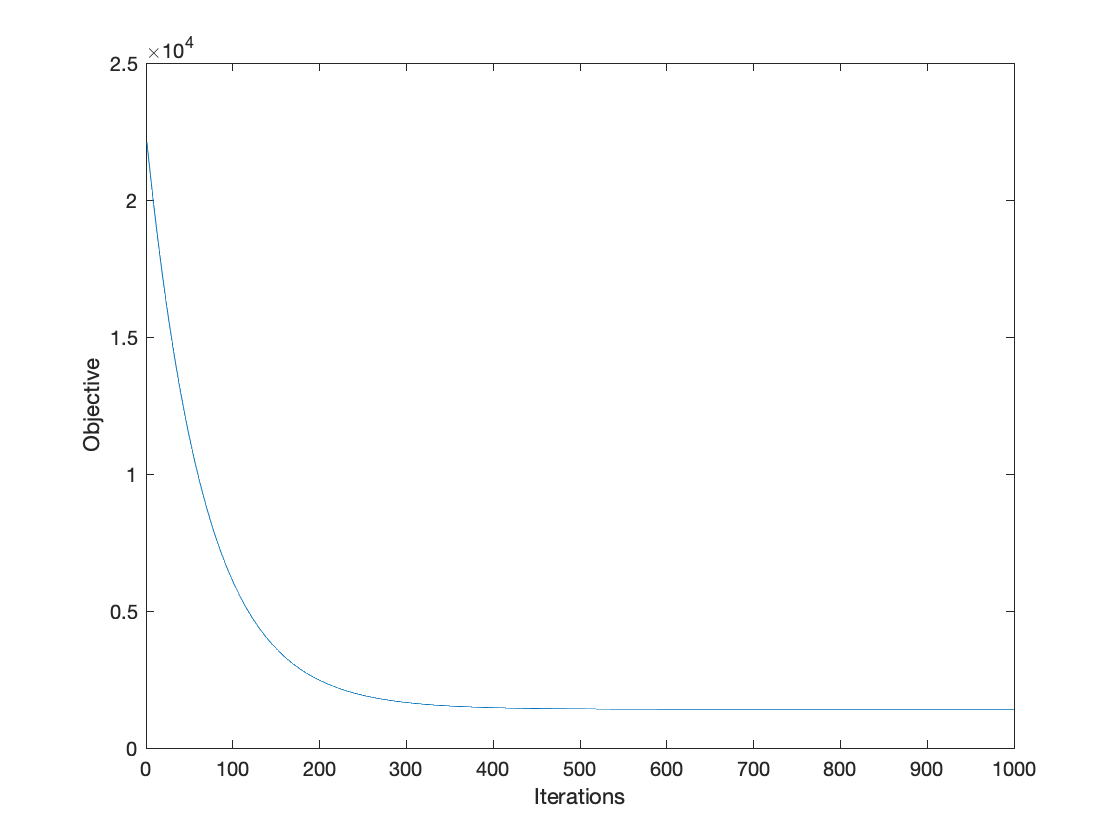
\includegraphics[width=0.8\linewidth]{fin_5.png}
	\caption{Decrease of $L(X,Y) = \frac{1}{2}\|X-Y\|_F^2+\|X\|_*$ with gradient descent.} % caption of the figure
	\label{fig:fig6}  % Label the figure so you can refer to it in text.
\end{figure}
\textbf{Codes (MatLab):}
\begin{verbatim}
Y = 5*rand(100,100);
X = 5*rand(100,100);
eta = 0.007;
l_L = [];

for i = [1:1000]
if rem(i,100) == 0
i
L(X,Y)
end
l_L = [l_L, L(X,Y)];

X_1 = X - eta * dLdX(X,Y);
X = X_1;
i = i+1;
end

plot(l_L)
xlabel('Iterations')
ylabel('Objective')

%%
function drv = dLdX(X,Y)
[U,S,V] = svd(X,0);
drv = (X - Y) + U * V';
end

function obj = L(X,Y)
obj = 1/2 * norm(X-Y, 'fro')^2 + norm(svd(X,0),1);
end
\end{verbatim}


\newpage
\section*{Problem 6 [20 pts]}
We turn to Logistic Regression:
\begin{equation}
	\min_\beta \sum\limits_{i=1}^{m} ln(1+e^{\lg \beta, \hat{x_i}\rg})-y_{i}\lg \beta, \hat{x_i}\rg, 
\end{equation}
where $\beta=(w;b), \hat{x}=(x;1)$. Assume $m=100, x\in\R^{99}$. Please randomly generate $x, y$ and find the optimal $\beta$ via 1) gradient descent; 2) Newton's method and 3) stochastic gradient descent (SGD) where the batch-size is 1. (need consider choosing appropriate  step-size if necessary). Change $m=1000, x\in\R^{999}$, observe which algorithm will decrease the objective faster in terms of iteration ($X$-axis denotes number of iteration) and CPU time. [You will receive another 5 bonus points if you implement backtracking line search]\\ \\
The objective function is $L(\beta,x_i,y_i) = ln(1+e^{\lg \beta, \hat{x_i}\rg})-y_{i}\lg \beta, \hat{x_i}\rg$.\\
In gradient method, we have the gradient:
\begin{equation}
	\begin{aligned}
		\frac{\partial L}{\partial \beta}=\frac{e^{<\beta,\hat{x_i}>}\hat{x_i}^T}{1+e^{<\beta,\hat{x_i}>}}-y_i\hat{x_i}^T
	\end{aligned}
\end{equation}
and: $\beta^{i+1}=\beta^i-\lambda\frac{\partial L}{\partial \beta}$. The decrease of $L$ with iterations is shown in the figure below.
\begin{figure}[H] % This is how figure are placed into latex document
	\centering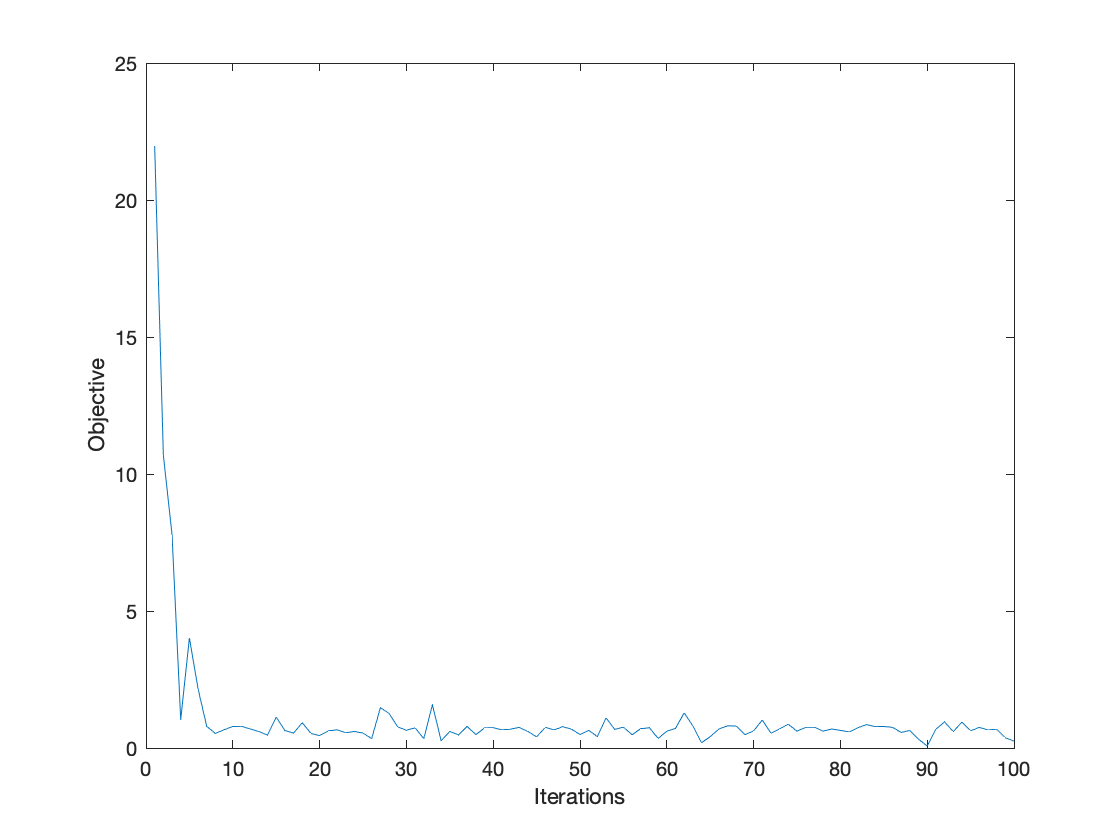
\includegraphics[width=0.6\linewidth]{fin_6_99_grd.png}
	\caption{Gradient descent (m=100, n=99).} % caption of the figure
	\label{fig:fig6}  % Label the figure so you can refer to it in text.
\end{figure}
In Newton's method, we have:
\begin{equation}
	\begin{aligned}
		\nabla&=\sum_{i=1}^m[p(x_i)-y_i]=X(p-y)\\
		H&=XWX^T 
	\end{aligned}
\end{equation}
, where $W$ is a diagonal matrix with the i-th diagonal element as $p(x_i)[1-p(x_i)]$. In each update, $w^{i+1}=w^i-H_i^{-1}\cdot\nabla$. The decrease of $L$ with iterations is shown in the figure below.
\begin{figure}[H] % This is how figure are placed into latex document
	\centering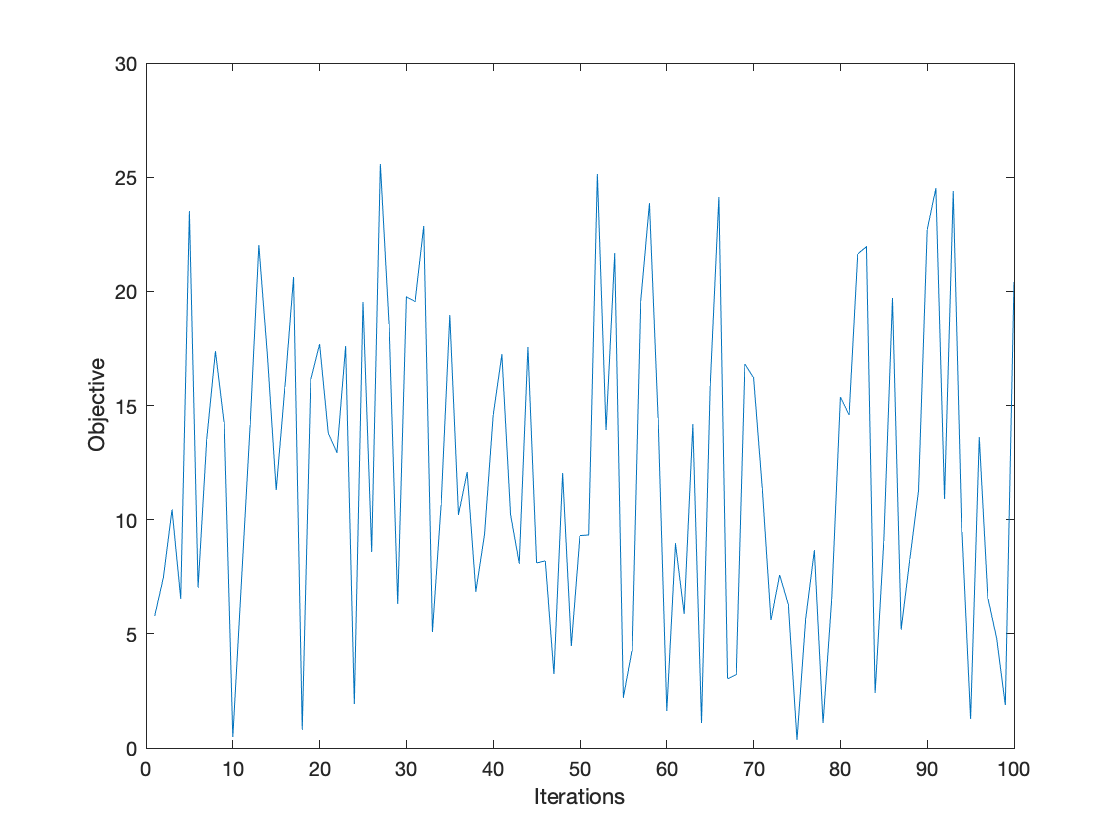
\includegraphics[width=0.6\linewidth]{fin_6_99_newton.png}
	\caption{Newton's method (m=100, n=99).} % caption of the figure
	\label{fig:fig6}  % Label the figure so you can refer to it in text.
\end{figure}
\textbf{Note: }In Newton's method, the objective function can reach very low values, but will then increase. The performance of Newton's method is not ideal in this case.\\
In SGD, we have:
\begin{equation}
	\begin{aligned}
		g=\frac{\partial L}{\partial w}&=(p(x_i)-y_i)x_i
	\end{aligned}
\end{equation}
and for each update $w^{i+1}=w^i-\alpha g$. The decrease of $L$ with iterations is shown in the figure below.
\begin{figure}[H] % This is how figure are placed into latex document
	\centering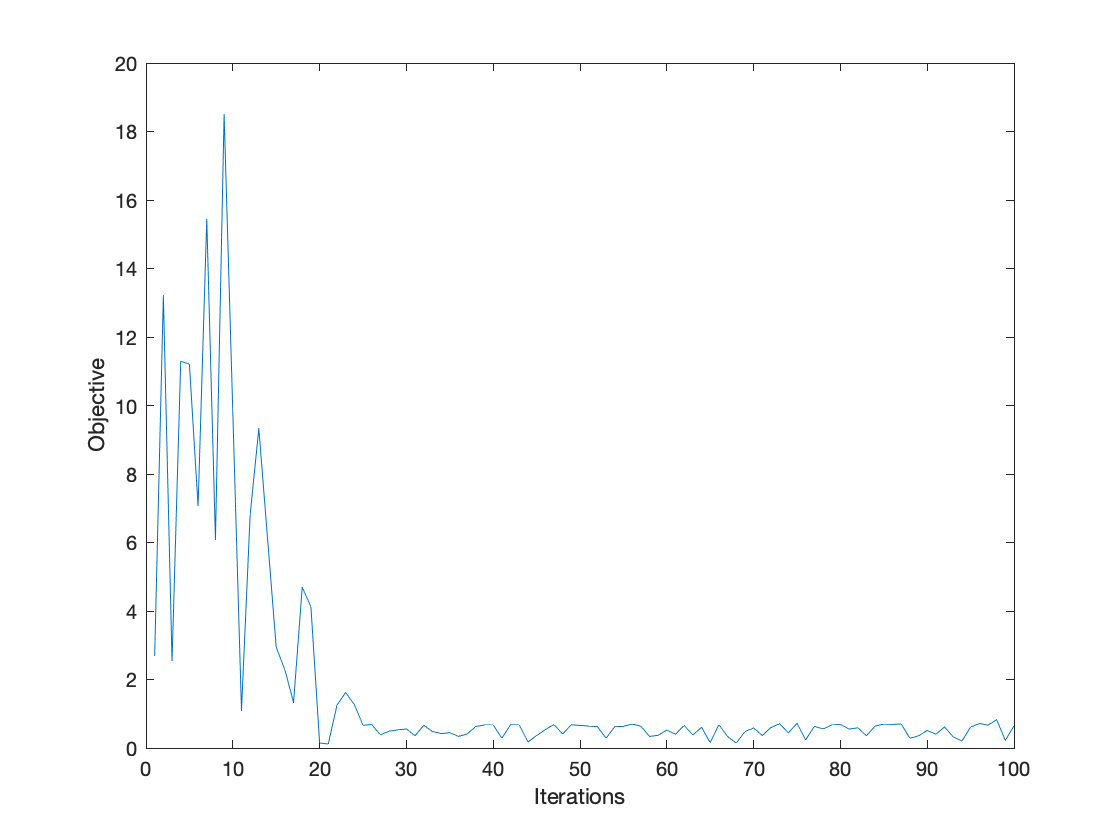
\includegraphics[width=0.6\linewidth]{fin_6 _99_sgd.png}
	\caption{SGD method (m=100, n=99, $\alpha$ = 0.1).} % caption of the figure
	\label{fig:fig0}  % Label the figure so you can refer to it in text.
\end{figure}
From the above results, we can see that the three methods in the order of fastest to slowest convergence is: gradient descent, SGD, Newton's method.
The time consumption of the three methods are: gradient descent - 0.01s, Newton's method - 0.29s, SGD - 0.01s. \\
In the case of $m=1000, n=999$, the decrease of $L$ with iterations is shown in the figures below.
\begin{figure}[H] % This is how figure are placed into latex document
	\centering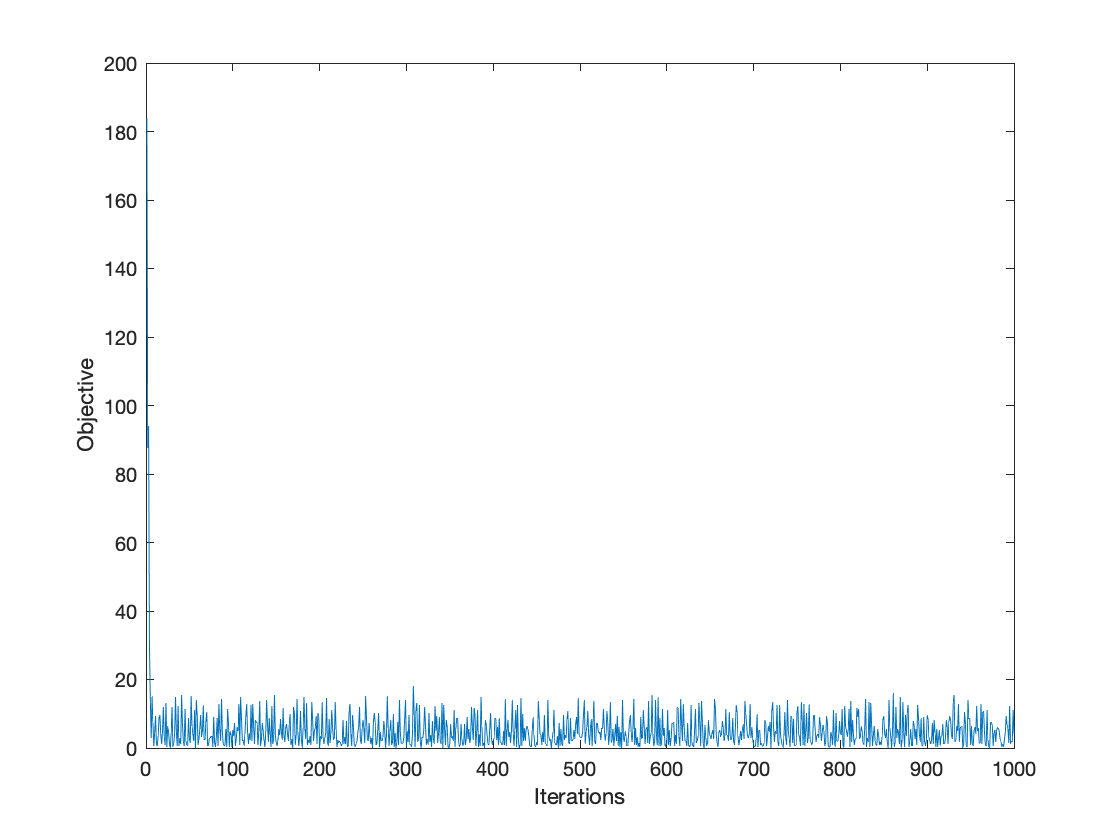
\includegraphics[width=0.6\linewidth]{fin_6_999_grd.png}
	\caption{Gradient descent (m=1000, n=999).} % caption of the figure
	\label{fig:fig6}  % Label the figure so you can refer to it in text.
\end{figure}
\begin{figure}[H] % This is how figure are placed into latex document
	\centering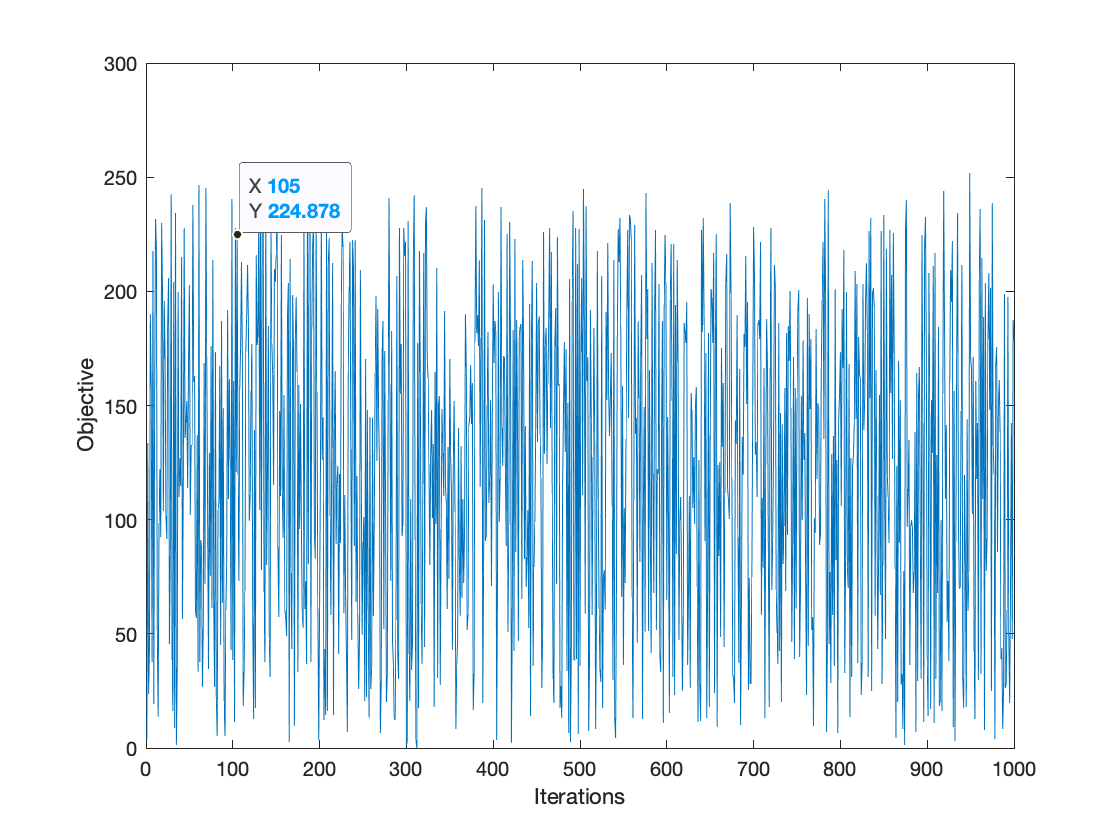
\includegraphics[width=0.6\linewidth]{fin_6_999_newton.png}
	\caption{Newton's method (m=1000, n=999).} % caption of the figure
	\label{fig:fig6}  % Label the figure so you can refer to it in text.
\end{figure}
\begin{figure}[H] % This is how figure are placed into latex document
	\centering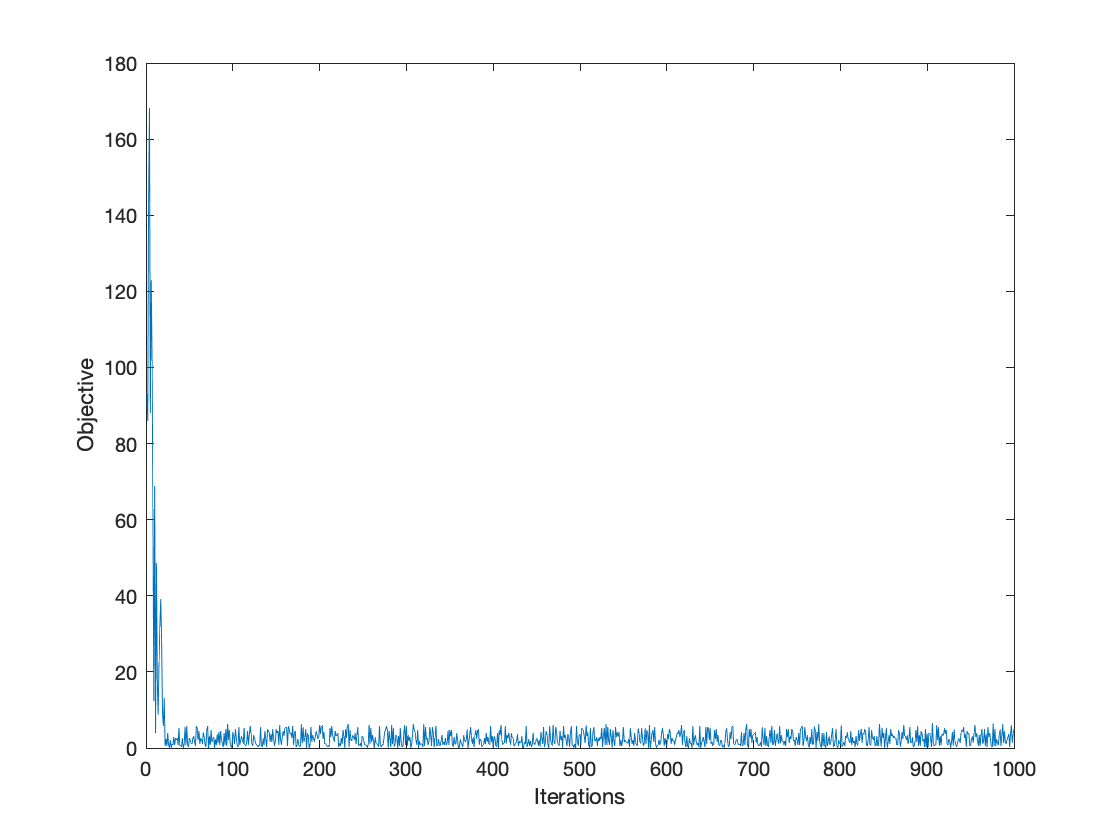
\includegraphics[width=0.6\linewidth]{fin_6 _999_sgd.png}
	\caption{SGD method (m=1000, n=999, $\alpha$ = 0.1).} % caption of the figure
	\label{fig:fig0}  % Label the figure so you can refer to it in text.
\end{figure}
From the above results, we can see that when $m, n$ are increased, the three methods in the order of fastest to slowest convergence is: gradient descent, SGD, Newton's method.
The time consumption of the three methods with increased $m,n$ are: gradient descent - 0.04s, Newton's method - 187.81s, SGD - 0.02s. \\\\
\textbf{Codes (MatLab): }
\begin{verbatim}
	clear all;
	
	m = 1000;
	n = 999;
	
	y = rand(1,m);
	w = rand(n,1);
	x = [w; rand]
	beta = [w; rand];
	lambda = 0.1;
	l = [];
	
	%%Grd descent
	% t = cputime;
	% for i = [1:m]
	%     x_i = [rand(n,1); 1];
	%     y_i = y(i);
	%     beta = beta - dLdb(beta,x_i,y_i) * lambda;
	%     obj = L(beta,x_i,y_i);
	%     l = [l, obj];
	% end
	% e = cputime - t;
	% disp('GD')
	% disp(n)
	% disp(e)
	
	
	%Newtons method
	
	% X = [rand(m,n), ones(m,1)];
	% p_vec = zeros(1,m);
	% 
	% t = cputime;
	% for i = [1:m]
	%     x_i = X(i,:);
	%     y_i = y(i);
	%     
	%     px_i = pxi(beta, x_i);
	%     obj = L(beta,x_i,y_i);
	%     grd = x_i * (px_i - y_i);
	%     
	%     W = zeros(m,m);
	%     for i = [1:m]
	%        W(i,i)=pxi(beta, X(i,:));
	%     end
	%     hes = X' * W * X;
	%     beta = beta - pinv(hes) * grd';
	%     
	% %     for i = [1:m]
	% %         p_vec(i) = pxi(beta, x_i);
	% %     end
	% %     grd = X' * (p_vec - y)';
	% %     
	% %     W = zeros(m,m);
	% %     for i = [1:m]
	% %        W(i,i)=pxi(beta, X(i,:));
	% %     end
	% %     hes = X' * W * X;
	% %     beta = beta - inv(hes) * grd;
	% 
	%     l = [l, obj];
	% end
	% e = cputime - t;
	% disp('Newton')
	% disp(n)
	% disp(e)
	
	%%SGD
	
	t = cputime;
	alpha = 0.1;
	for i = [1:m]
	y_i = y(i);
	x_i = [rand(n,1); 1];
	px_i = pxi(beta, x_i);
	g = (px_i - y_i) * x_i;
	beta = beta - alpha * g;
	obj = L(beta,x_i,y_i);
	l = [l, obj];
	end
	e = cputime - t;
	disp('SGD')
	disp(n)
	disp(e)
	
	%% Test
	
	%%
	plot(l)
	xlabel('Iterations')
	ylabel('Objective')
	%%
	function obj = L(beta,x_i,y_i)
	obj = log(1 + exp(dot(beta' , x_i))) - y_i * dot(beta' , x_i);
	end
	
	%%
	function grd = dLdb(beta,x_i,y_i)
	grd = exp(dot(beta' , x_i))/(1 + exp(dot(beta' , x_i))) - y_i * x_i;
	end
	
	%%
	function likelihood = pxi(beta, x_i)
	likelihood = 1/(1+exp(-dot(beta', x_i)));
	end
\end{verbatim}


\newpage
\section*{Problem 7 [10 pts]}
Please design an (either toy or real-world) experiment  to demonstrate that PCA can be helpful for denoising.\\\\
Take a 480*360 picture of a snowy owl as an example.
\begin{figure}[H] % This is how figure are placed into latex document
	\centering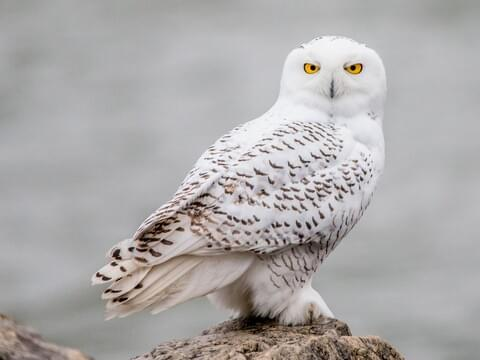
\includegraphics[width=0.6\linewidth]{snowy_owl.jpg}
	\caption{Original picture.} % caption of the figure
	\label{fig:fig6}  % Label the figure so you can refer to it in text.
\end{figure}
Add Gaussian noise with $\mu=0, \sigma=0.1$ to all three RGB channels, we have a noisey image.
\begin{figure}[H] % This is how figure are placed into latex document
	\centering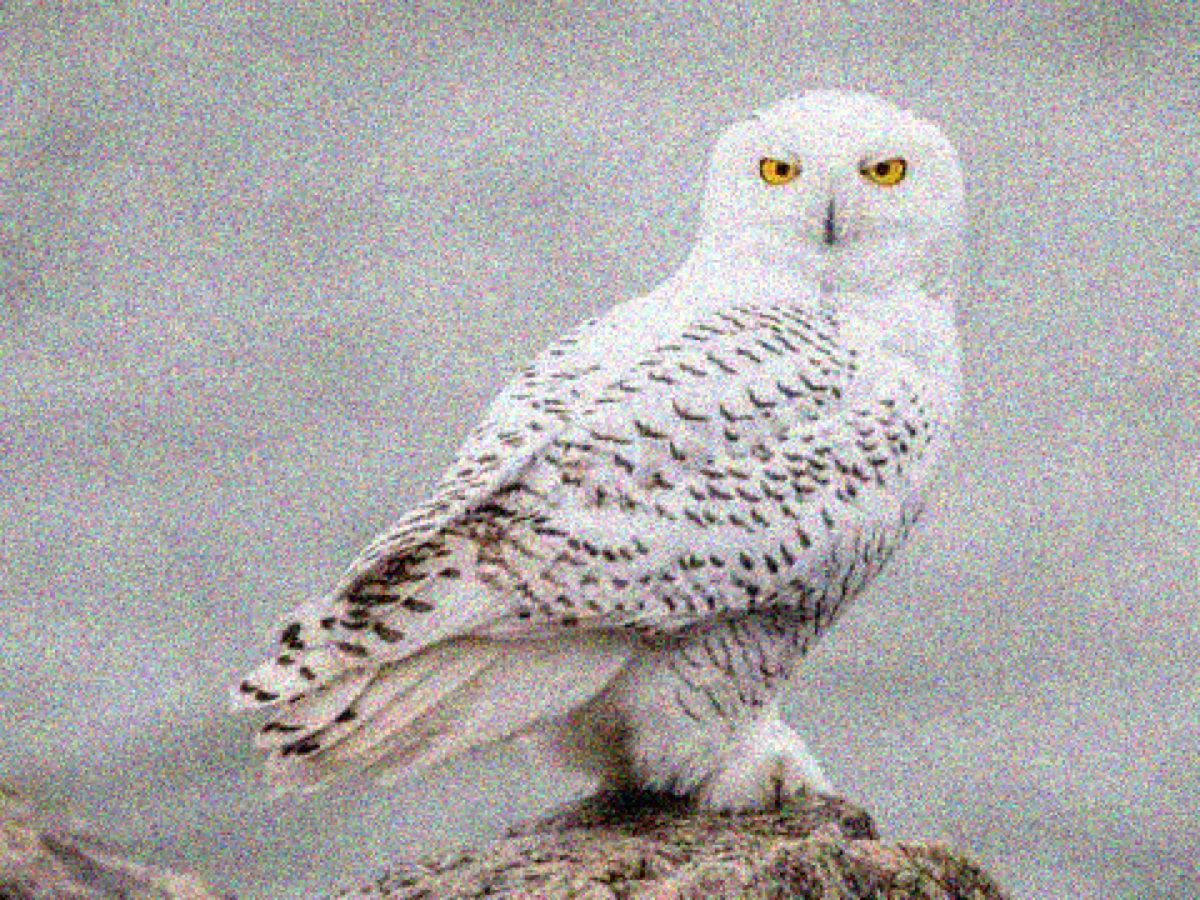
\includegraphics[width=0.6\linewidth]{snowy_owl_noisey.png}
	\caption{Noisey picture.} % caption of the figure
	\label{fig:fig6}  % Label the figure so you can refer to it in text.
\end{figure}
Performing PCA on the noisey picture with the first 100 PCs, we have a reconstructed picture.
\begin{figure}[H] % This is how figure are placed into latex document
	\centering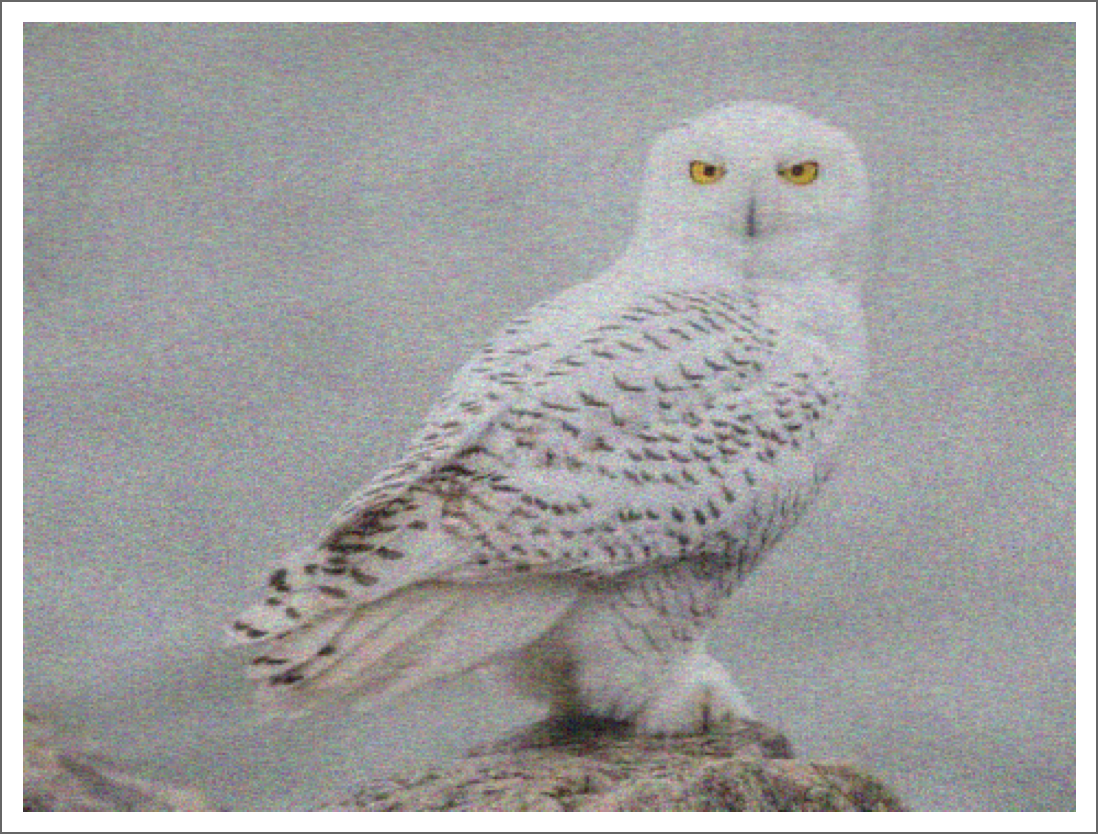
\includegraphics[width=0.6\linewidth]{snowy_owl_recon.png}
	\caption{Reconstructed picture.} % caption of the figure
	\label{fig:fig6}  % Label the figure so you can refer to it in text.
\end{figure}
We can see that the noises in the reconstructed picture are smoothed out.\\\\
\textbf{Codes (Mathematica):}
\begin{verbatim}
	cwd = NotebookDirectory[];
	{m, n} = Import[cwd <> "snowy_owl.jpg", "ImageSize"];
	original = Import[cwd <> "snowy_owl.jpg"];
	noisey = ImageEffect[original, {"GaussianNoise", 0.1}]
	pxl = N[Flatten[ImageData[noisey], 1]];
	mean = Mean[pxl];
	pxlCtr = # - mean & /@ pxl;
	(*RGB channels*)
	R = ArrayReshape[pxlCtr[[All, 1]], {m, n}]; G = 
	ArrayReshape[pxlCtr[[All, 2]], {m, n}]; B = 
	ArrayReshape[pxlCtr[[All, 3]], {m, n}];
	
	(*Reconstruction single channel*)
	
	recon[channel_, nPC_] := Module[{u, s, v, picrecon},
	(*SVD*){u, s, v} = SingularValueDecomposition[channel];
	(*Reconstruction using nPC columns*)
	picrecon = 
	u[[All, ;; nPC]].s[[;; nPC, ;; nPC]].Transpose[v[[All, ;; nPC]]];
	picrecon]
	(*Reconstruct 3 channels*)
	
	reconRGB[nPC_] := 
	ArrayReshape[
	Transpose[
	Flatten /@ {recon[R, nPC], recon[G, nPC], recon[B, nPC]}], {n, m, 
		3}]
	rgbPlot[plot_] := 
	ArrayPlot[ArrayReshape[plot, {n, m, 3}], 
	ColorFunction -> Function[p, RGBColor[p[[1]], p[[2]], p[[3]]]], 
	ColorFunctionScaling -> True]
	
	rgbPlot[reconRGB[#]] & /@ {100}
\end{verbatim}


\newpage
\section*{Bonus Problem 8 [10 pts]}
\begin{equation}
	\text{\bf Solve:} \quad \min \|\vx\|_{0} \quad \mbox{s.t.}\quad { \mA \vx = \vy. }
\end{equation}
We have proved that if $\vy = \mA \vx_o$ with
\begin{equation}\label{krank}
	\|\vx_o\|_0 \; \le \; \tfrac{1}{2} \, \mathrm{krank}(\mA).
\end{equation}
Then $\vx_o$ is the unique optimal solution to the  $\ell^0$ minimization problem\index{$\ell^0$ minimization}
\begin{equation}
	\min \|\vx\|_{0} \quad \mbox{s.t.}\quad { \mA \vx = \vy. }
\end{equation}
However, when $\mA$ is of size $5 \times 12$, the following figure illustrates the fraction of success across 100 trials.
\begin{figure}[h!]
	\centering
	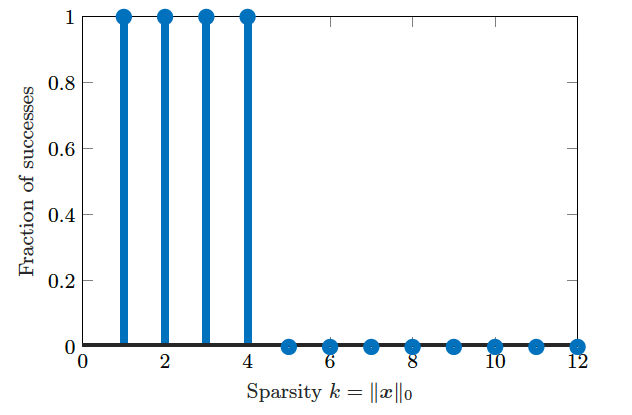
\includegraphics[width=7cm]{simulation-L0.png}
	% \caption{Caption}
	% \label{fig:my_label}
\end{figure}    
Apparently $krank(\mA)\le rank(\mA)\le 5$, therefore, when sparsity $k=1, 2$ satisfying Eq. (\ref{krank}) it has $100\%$ recovery success rate is not surprising. However, the above experiment also shows even $k=3, 4$ which violates Eq. (\ref{krank}), still it can be recovered at $100\%$. Please explain this phenomenon.
%\textbf{Proof:} $
%\mb A \mb \hat{\mb x} = \y \Rightarrow \mb A \left( \hat{\mb x} - \x_o \right) = \mb A \hat{\mb x} - \mb A \x_o = \mb y - \mb y \; = \; \mb 0.$
\end{document}
